\section*{2.1 Identify the ciphertexts}

The ciphertext that comes from AES is a modern algorithm and works on bytes.
Older algorithms works on words and letters and changes these in some way.
In my case I can clearly see that `0.txt` has random characters in it, while the rest has letters.
None of the other texts look very much like plain English, but some do have some characteristic similarities.
Therefore `0.txt` comes from AES and will be put aside until later.

\subsection*{1.txt}

This text has some quotation marks as well as a question mark.
Also the words look like they have lengths like english words.

The frequency of letters in the histogram in Figure \ref{fig:1freq} of this text shows a distribution which closely corresponds to the distribution of letters in the english language\cite{frequencies} if variance is taken into account.
However the most popular letters doesn't match up with the english ones.

In a random simple substitution each letter in an alphabet is mapped to a random other letter in another alphabet.
For instance all As can be switched with Zs and all Cs with Qs and so forth.
Because of this the distribution of letters should stay the same, but there should be random what letters have which percentage of the total amount of letters.
This corresponds nicely with this histogram.

The diagram of this text shown in Figure \ref{fig:1diagram} differes from the usual frequencies in the english language shown \cite{diagraphs}.
However this does not neccesarily mean that there is no correlation here, the variance in such a small text is huge.
The difference between each of the diagraphs is still much the same.

The autocorrelation did not show any significant periods or similar in this case, and I chose not to include it.
This is not only because the graph seemed to have random matches all over the place, but also because the other two analysis have given me enough evidence to be certan of what is going on.

Therefore I believe that this ciphertext has been made with a random simple substitution, and some easy testing with the tools verify this.

\begin{figure}[ht!]
    \begin{center}
        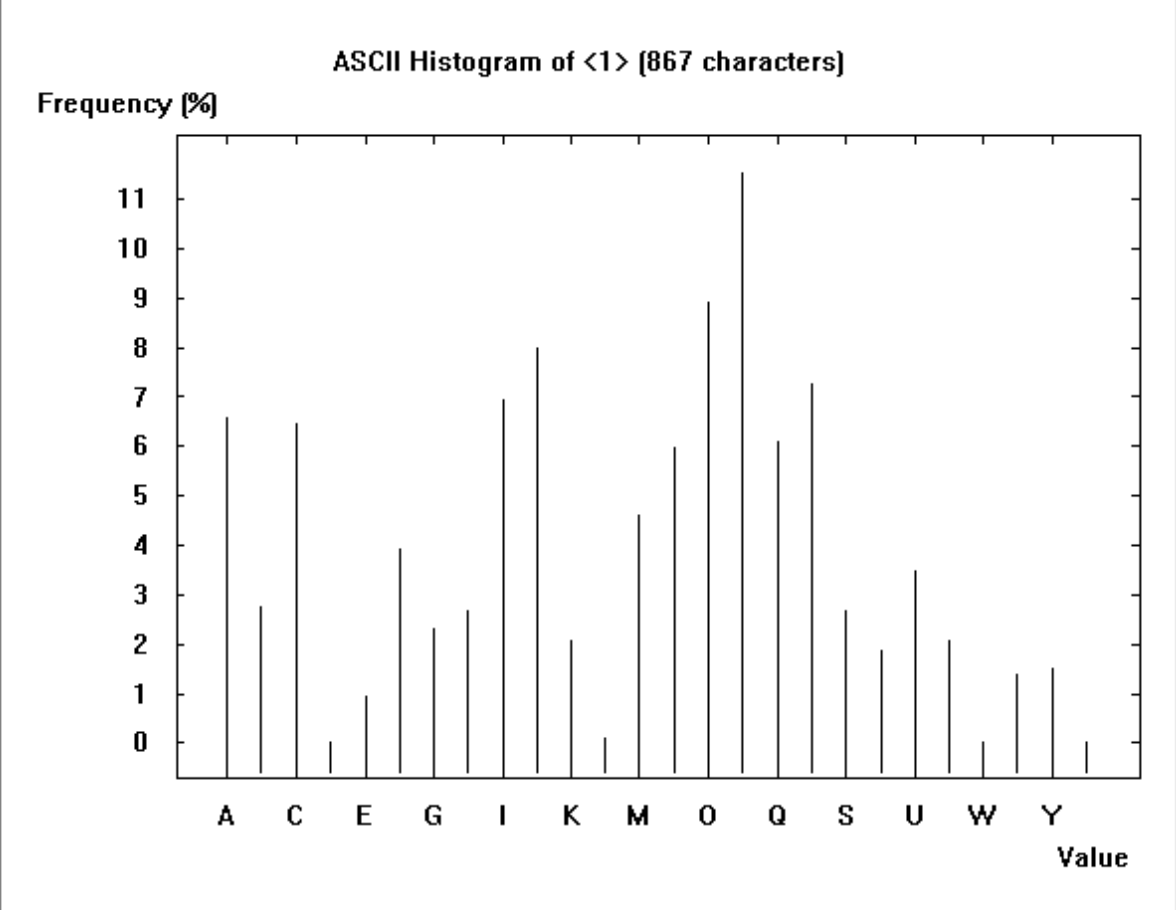
\includegraphics[width=0.7\textwidth]{assets/1_frequency.png}
        \caption{Frequency for text 1}
        \label{fig:1freq}
    \end{center}
\end{figure}

\begin{figure}[ht!]
    \begin{center}
        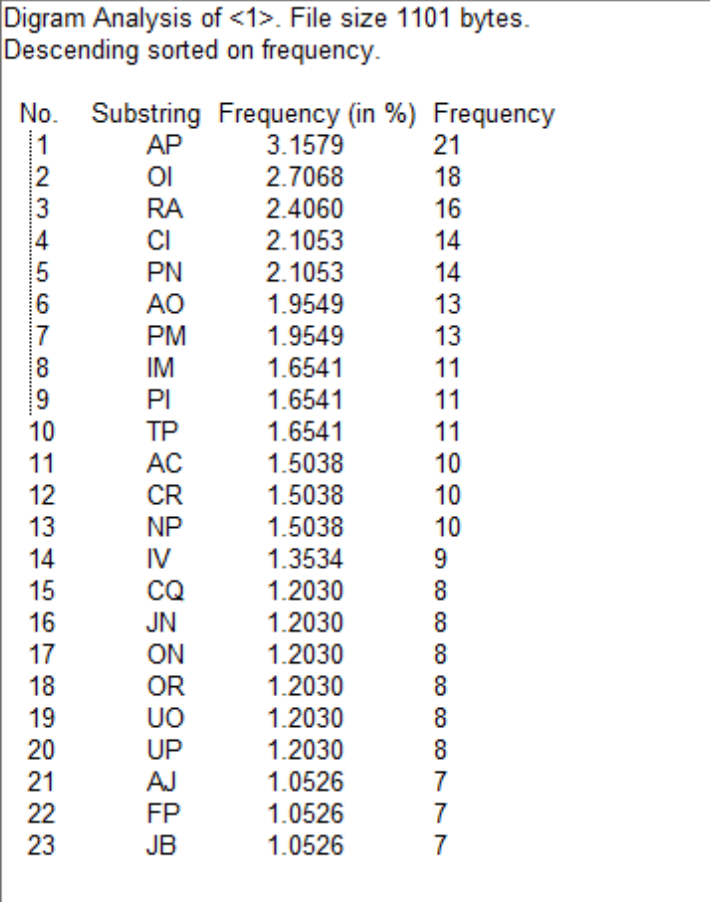
\includegraphics[height=0.8\textwidth]{assets/1_diagram.png}
        \caption{Diagram for text 1}
        \label{fig:1diagram}
    \end{center}
\end{figure}

\newpage
\subsection*{2.txt}

This text is one long sentence and the words doesn't really look like the lengths of english words.

One can see from the histogram in 2.txt (Figure \ref{fig:2freq}) that the distribution of letters closely resembles the distribution in the english language with corresponding letters.

In a transposition the letters themselves doesn't change, but rather the technique for reading said letters change.
The idea here is to give a permutation of the plaintext and thereby obscure the contents.

Since this doesn't change the distribution of the letters at all, it will still correspond to the common distribution of letters in the language it's written in.

The diagram for this text shown in Figure \ref{fig:2diagram} has not the most common diagraphs in the english language\cite{diagraphs}.
If this indeed is a transposition then the diagraphs should not match up.
The frequency chart is the one that really makes a difference here.

As with the previous text I choose here not to include the autocorrelation graph.
Just as the last one it seemed to be random all over the place.

This all together makes me believe that this ciphertext has been made with transposition.

\begin{figure}[ht!]
    \begin{center}
        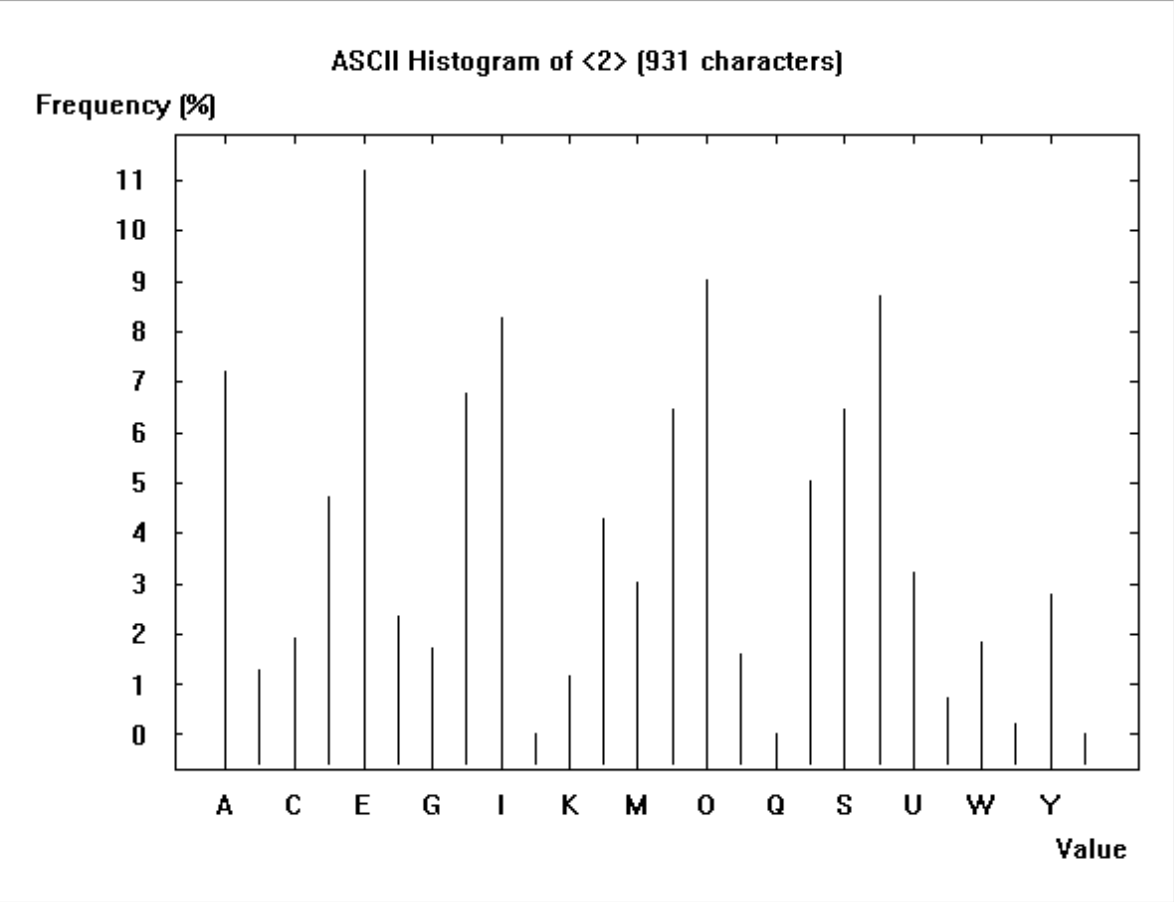
\includegraphics[width=0.7\textwidth]{assets/2_frequency.png}
        \caption{Frequency for text 2}
        \label{fig:2freq}
    \end{center}
\end{figure}

\begin{figure}[ht!]
    \begin{center}
        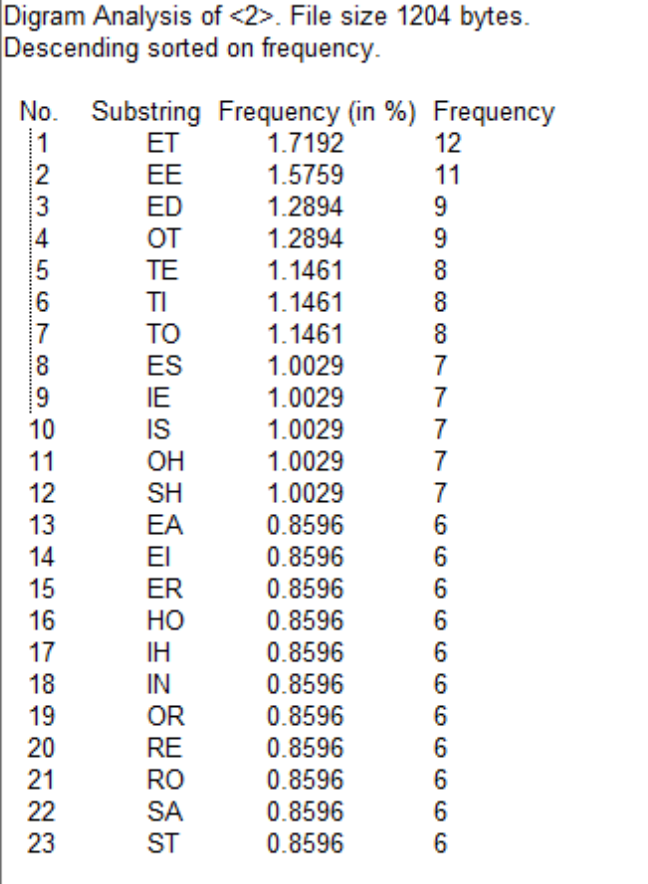
\includegraphics[height=0.7\textwidth]{assets/2_diagram.png}
        \caption{Diagram for text 2}
        \label{fig:2diagram}
    \end{center}
\end{figure}

\newpage
\subsection*{3.txt}

This text has some quotation marks and some words with lengths that might be english.

The distribution of the histogram for 3.txt in Figure \ref{fig:3freq} has a different distribution than previously seen.
This distribution is much flatter where all the letters are closer to the mean value.
One can therefore rule out transposition and simple substitution.

This flattening of the distribution can point to polyalphabetic substitution or some other way of flatten the distribution.
Vigenère cipher is one form of polyalphabetic substitution.
My initial thought was therefore that this should be the Vigenêre cipher.
However if we examine the autocorrelation seen in Figure \ref{fig:3autocorr} of this cipher we see no significant spikes in the graph.
This means that the text is not Vigenère.

The diagraph frequencies here is not that interesting based on the other facts we have gathered.
We can observe that they seem to have a somewhat correlation to what we might expect.

Based on these facts I therefore believe this ciphertext is made by 2 x 2 Hill cipher.

\begin{figure}[ht!]
    \begin{center}
        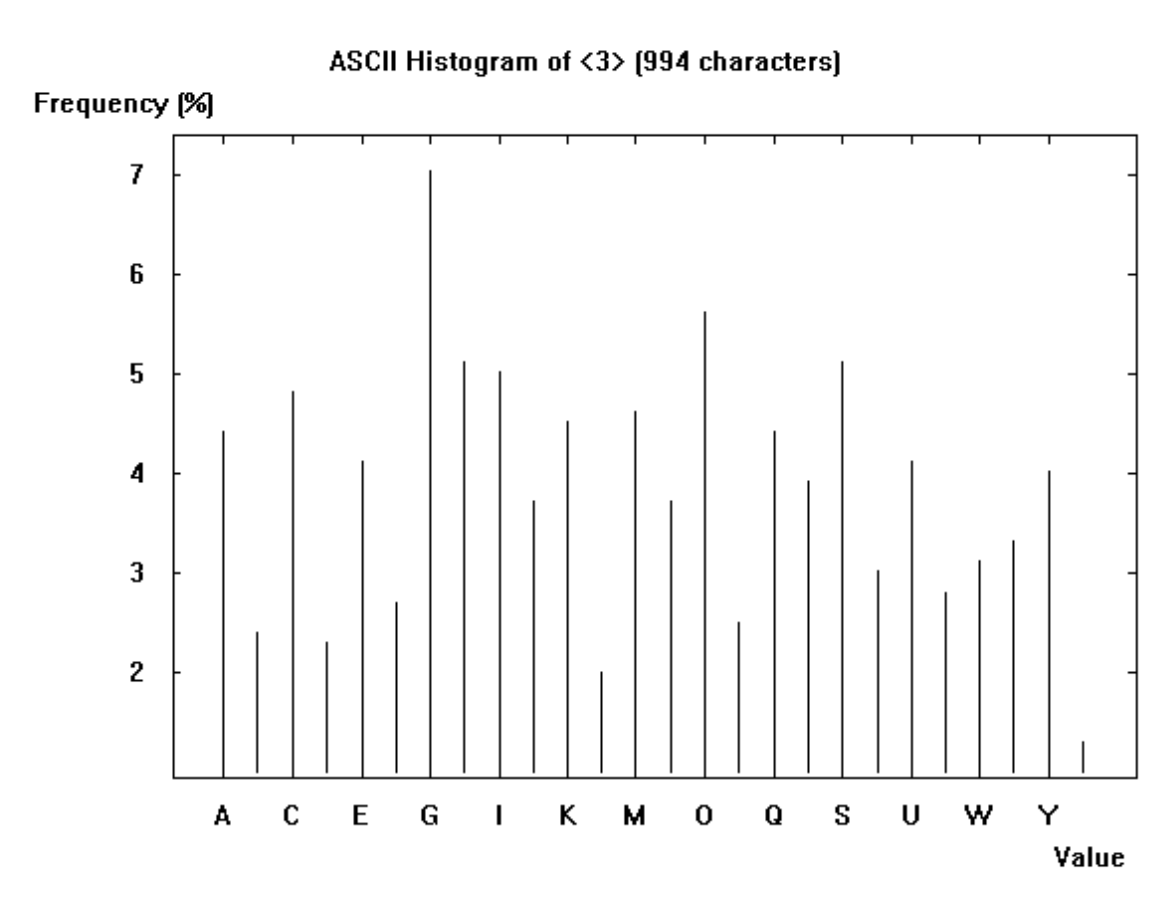
\includegraphics[width=0.8\textwidth]{assets/3_frequency.png}
        \caption{Frequency for text 3}
        \label{fig:3freq}
    \end{center}
\end{figure}

\begin{figure}[ht!]
    \begin{center}
        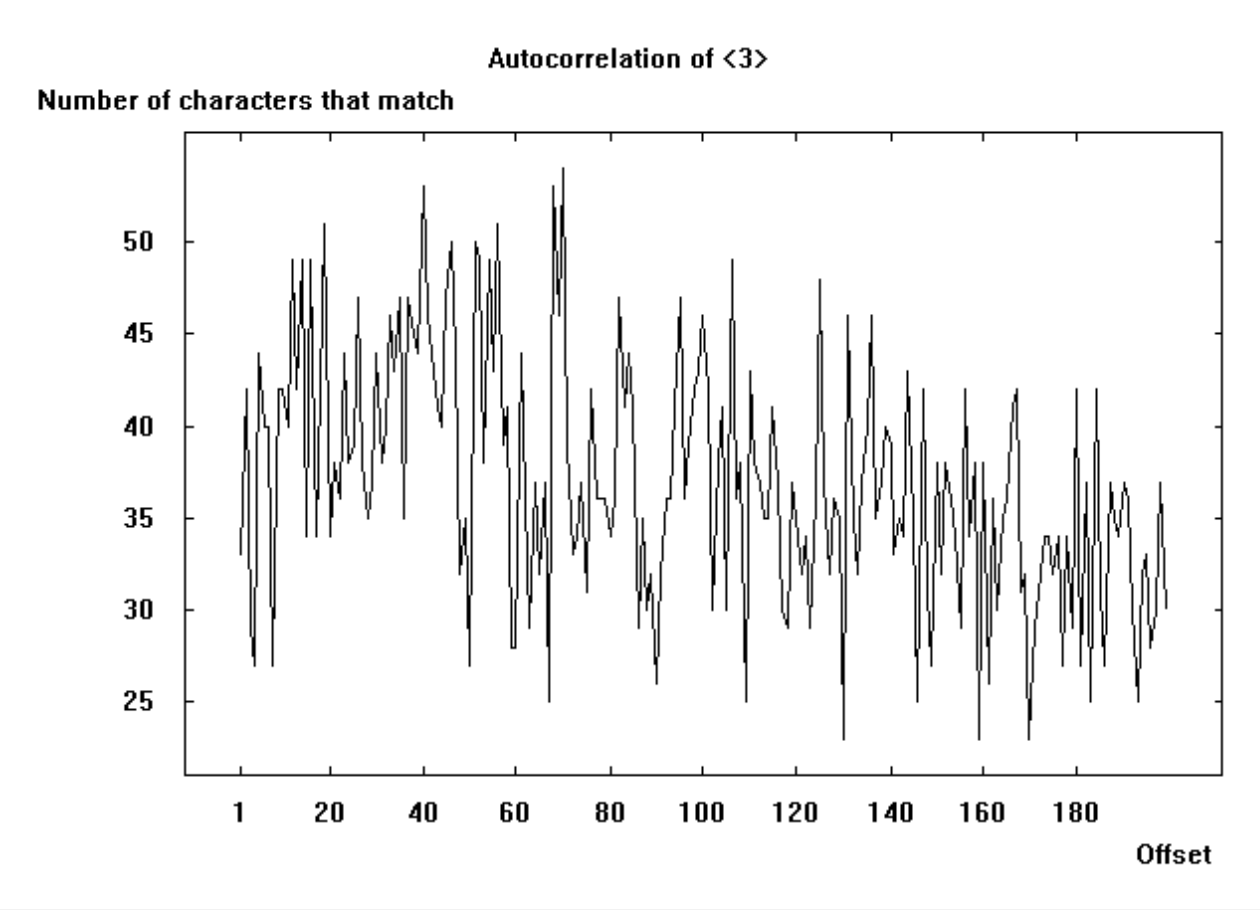
\includegraphics[width=0.8\textwidth]{assets/3_autocorr.png}
        \caption{Autocorrelation for text 3}
        \label{fig:3autocorr}
    \end{center}
\end{figure}

\newpage
\subsection*{4.txt}

This text doesn't really look like english at all.

The distribution for this text is shown in Figure \ref{fig:4freq}.
The initial thoguht here was that this could not be a polyalphabetic cipher because of too many letters away from the mean.
However this is, as all the other texts, a very short text, so the variance explodes.
The autocorrelation is what really stands out when this text is looked at.

Looking at Figure \ref{fig:4autocorr} we can clearly see a period here.
The pattern seem to repeat itself very periodically.
If we try to use the analysis tool in CrypTool to find Periodicity we find nothing, however.
This might be because of this tool being used wrongly by yours truly.

With all the information gathered the diagram aren't that interesting.

The autocorrelation itself is enough to think this is a Vigrène cipher, and some easy testing verifies this.

\begin{figure}[ht!]
    \begin{center}
        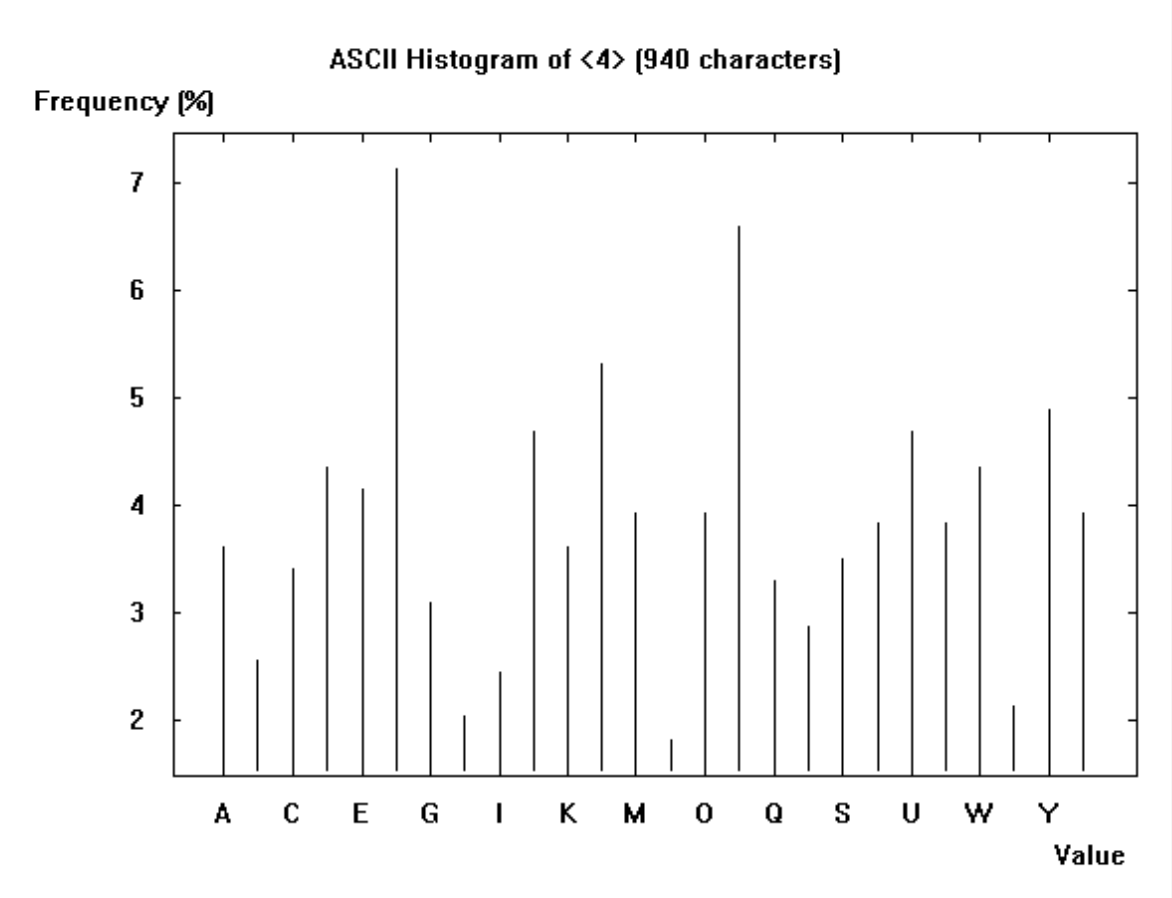
\includegraphics[width=0.8\textwidth]{assets/4_frequency.png}
        \caption{Frequency for text 4}
        \label{fig:4freq}
    \end{center}
\end{figure}

\begin{figure}[ht!]
    \begin{center}
        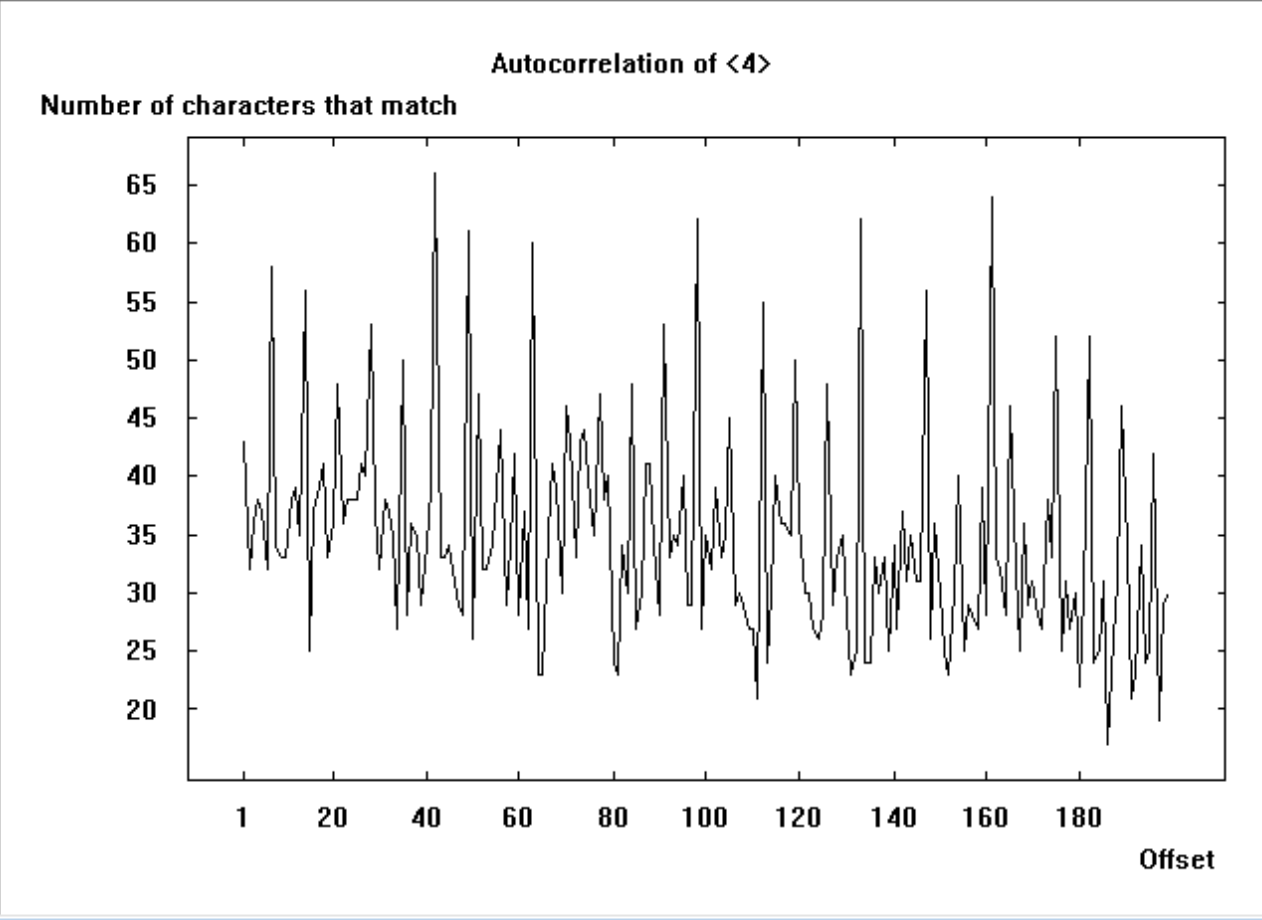
\includegraphics[width=0.8\textwidth]{assets/4_autocorr.png}
        \caption{Autocorrelation for text 4}
        \label{fig:4autocorr}
    \end{center}
\end{figure}

\section*{2.2 Obtaining the plaintexts}

For the random simple substitution I used the recognition based on the most used frequent words of a language.
I believed this to be the most effective one because of the shortness of the text, since diagraphs and so on can very based on a short text.
I used e as the most frequent character, since I had seen a character in the frequency be a lot more common than the rest.
The initial result was very good, and I looked for words I knew based on the surrounding words for the final letters.
This text is from Sherlock Holmes.

The key is OYHMPBVAC*EFGIJKLNQRSTU*X*.
The finished text is: \\
"Had he ever spoken of Swandam Lane?"
"Had he ever showed any signs of having taken opium?"
"Thank you, Mrs. St. Clair. Those are the principal points about
which I wished to be absolutely clear. We shall now have a little
supper and then retire, for we may have a very busy day 
A large and comfortable double-bedded room had been placed at our
disposal, and I was quickly between the sheets, for I was weary
after my night of adventure. Sherlock Holmes was a man, however,
who, when he had an unsolved problem upon his mind, would go for
days, and even for a week, without rest, turning it over,
rearranging his facts, looking at it from every point of view
until he had either fathomed it or convinced himself that his
data were insufficient. It was soon evident to me that he was now
preparing for an all-night sitting. He took off his coat and
waistcoat, put on a large blue dressing-gown, and then wandered
about the room collecting pillows from his bed and cushions from
the sofa and armchairs. With these he constructed a sort of
Eastern divan, upon which he perched himself cross-legged, with



The Vigenère cipher was cracked using the analysis part that only said Vigenère and nothing else.
Cryptool found that the keylength was 7 and cracked the text.
The key is BLSRMHY.
This in spite of not finding any period beforehand.

The text is: \\
theRe iN tWeNTY MinUTes."
it WaS nearlY fOUR o'cLOck WheN We aT laST, afTeR PaSsIng ThRoUgh
The bEaUTifUL STROUd valLeY, aNd oVeR THe bROad GleaMinG SeVeRn,
FoUNd OURseLVes at The PrEtTY LiTTle cOUnTrY-TOWn Of rOSS. A
LeaN, ferReT-Like Man, fURTIve aNd sLy-lOOkiNg, WaS WaItiNg foR
uS UPOn The PLaTFoRM. In sPiTe Of THe lIghT broWN dUStcOaT aNd
leaThEr-leggiNgS WhicH he WORe In deferEnce TO hIs RUSTiC
sURROUNdiNgS, I Had NO diFficUlTY in RecoGniSing leSTRadE, of
scOTLand yarD. WiTh hiM we dROVE to The HErefORd ArmS WheRe a
ROOm Had aLReadY been Engaged FoR US.
"I have ORdeRed a carRiage," SaId LeSTrade aS We SaT OVer a cUP
Of TEa. "I KNeW YoUR eneRgeTic natURe, anD thaT YoU woULd nOt be
hapPy UNTil YoU had bEen ON ThE sceNe oF the cRiMe."
"IT Was VeRY NicE and cOmPliMenTarY Of YoU," HoLMes anSWeReD. "IT
IS enTiReLY a QueSTioN of baRoMeTRic pReSSURe."
leSTRadE loOKed StaRTleD. "I dO NOT QuiTe foLloW," he said.
"HOW iS the glaSs? tWenTY-niNe, I sEe. NO WinD, and NOT a clOUd
iN the SkY. i haVe a casefUl oF cigaReTteS herE whIch nEed
SMOkIng, aNd THe SOfa iS veRY mUCh SUPerIoR TO ThE uSUal cOunTRY
hOteL aboMinaTioN. I dO NOT ThiNK That iT iS pRobable ThaT I
Shall USe THe caRRiage TO-niGhT."

\section*{2.3 Brute force attack}

\subsection*{1. Perform brute force attack}

The brute force attack was carried out using CrypTool.
It was conducted on a MacBook Pro Retina late 2013 model with Windows 7 running in a VM using Parallels 9.

The successful run took 4 minutes and 51 seconds and 61 hundreds to run.
The key found was 7EEC908000...(etc with 0s) and the plaintext (like before capitalized to stand out): \\
THE ARNSWORTH CASTLE BUSINESS. A MARRIED WOMAN GRABS AT HER BABY;
AN UNMARRIED ONE REACHES FOR HER JEWEL-BOX. NOW IT WAS CLEAR TO
ME THAT OUR LADY OF TO-DAY HAD NOTHING IN THE HOUSE MORE PRECIOUS
TO HER THAN WHAT WE ARE IN QUEST OF. SHE WOULD RUSH TO SECURE IT.
THE ALARM OF FIRE WAS ADMIRABLY DONE. THE SMOKE AND SHOUTING WERE
ENOUGH TO SHAKE NERVES OF STEEL. SHE RESPONDED BEAUTIFULLY. THE
PHOTOGRAPH IS IN A RECESS BEHIND A SLIDING PANEL JUST ABOVE THE
RIGHT BELL-PULL. SHE WAS THERE IN AN INSTANT, AND I CAUGHT A
GLIMPSE OF IT AS SHE HALF-DREW IT OUT. WHEN I CRIED OUT THAT IT
WAS A FALSE ALARM, SHE REPLACED IT, GLANCED AT THE ROCKET, RUSHED
FROM THE ROOM, AND I HAVE NOT SEEN HER SINCE. I ROSE, AND, MAKING
MY EXCUSES, ESCAPED FROM THE HOUSE. I HESITATED WHETHER TO
ATTEMPT TO SECURE THE PHOTOGRAPH AT ONCE; BUT THE COACHMAN HAD
COME IN, AND AS HE WAS WATCHING ME NARROWLY IT SEEMED SAFER TO
WAIT. A LITTLE OVER-PRECIPITANCE MAY RUIN ALL."
"AND NOW?" I ASKED.
"OUR QUEST IS PRACTICALLY FINISHED. I SHALL CALL WITH THE KING
TO-MORROW, AND WITH YOU, IF YOU CARE TO COME WITH US. WE WILL BE
SHOWN INTO THE SITTING-ROOM TO WAIT FOR THE LADY, BUT IT IS
PROBABLE THAT WHEN SHE COMES SHE MAY FIND NEITHER US NOR THE
PHOTOGRAPH. IT MIGHT BE A SATISFACTION TO HIS MAJESTY TO REGAIN

\subsection*{2. Estimations}

The amount of possible keys to check with an effective key of 28 bits is $2^{28} = 268 435 456$.
When the key is reduced to 24 bits, which is a 4 bit reduction, the possible outcomes is reduced by a factor of $2^{4} = 16$.
With only $2^{28-4} = 2^{24} = 16 777 216$ possible keys the search the time it takes to brute-force search should also be reduced by a factor of 16.
The total time it took to calculate the 28 bit key is 291.61 seconds.
My estimate is therefore:
$$ \frac{291.61 \text{ sec}}{16} = 18.22 \text{ sec} $$
The total amount of time to search for a 24 bit key should take 18.22 seconds.

The actual time taken to find a 24 bit key was 18 seconds and 97 hundreds, which is not so far off from our estimate.
The error in my estimate is $4 \%$ off, which is about as good as an estimate gets.
Every run of the brute-force search will have some variance.
Personally I think the estimate is very good.

To estimate the time it will take to find a 128 bit key we calculate the same way as before.
The possible outcomes is now $2^{100}$ times bigger than before.
So we increase the time it took to find a 28 bit key by $2^{100}$ and we have our estimate.

$$ 291.61 \text{ sec } \cdot 2^{100} = 1.172 \cdot 10^{25} \text{ years} $$

\section*{2.4 Avalanche effects in AES}

\subsection*{SubBytes and ShiftRows}

The SubBytes step of AES replaces each byte with another byte based on a lookup table called the Rijndael S-box.
Different from DES this box is the same for all bytes.
The mathematics behind the substitution is a two step process.
The first step is to transform each bit into a polynomial vector, where a $1$ in the $n\text{-th}$ position would become an $x^{n}$.
With this polynomial you are to compute the inverse of this matrix with the respect to 1 modulo some irreductible polynomial, which one can draw parallels to a prime number, but for a field.
After you aquire the inverse, you are to do an affine transformation to get your final result.
This 1 to 1 mapping is constant for each possible input.

The ShiftRows section of the shufles the bytes to different locations.
If you visualize a 4 by 4 matrix, each row is shiften $n$ times to the left with wrapping if the top row is index 0.
This makes it so that a change in one 4 byte block will have an effect on the rest of the blocks for the next step.

After the first two steps of the first round a lot of the blocks is 63.
This is because the first step is a 1 to 1 mapping, which is constant for each input and then they are shifted.
Until this stage no change has happened which can make a same character byte map to multiple outputs.
The reason for not all cells to be 63 is that the initial step is to XOR the input with the key before round 1.

\subsection*{Second round}

After SubBytes and ShiftRows in the round 2, all but [(0,0), (1,3), (2,2), (3,1)] remain unchanged.
This is unaffected by the input from the first input byte and has been verified by empiric testing.

The reason for this is that we have run MixColumns one time.
MixColumns use a predefined matrix to give its output.
This matrix says how much each input will change the output.
Therefore one bit change in one input to MixColumns will change every output from that collection of 4 bytes.

In our example that means that the elements of the first column will change before round two.
In round two, as we know, we will get a 1 to 1 mapping first and a shift.
The shift makes the first column go into the exact same places as we noticed change.

This is the reason only these cells change, but it is also a good example of one small input change leads to a big output change (16 bit change in output from <4 input change in input).

\subsection*{Bottom right byte}

If the bottom right byte is changed the key will change.
In the first round row 2 (indexed from 0) and the bottom right byte will change.
The last key will fully change if this byte is changed in the key.
If however the 3rd column is changed instead of the 4th, a lot less change will occure in the key.

This is because the next key generator is based on having each 4th column rotated (RotWord) as well as SubByted.
After this it is XORed with the column before as well as a constant.
All other rows are XORed with the row 4 places back.

This makes an entropy that gradually increases with each round.

The avalanche effect is that a small change in input gives a large change in output.
Each part of AES does this directly or indirectly.
